
%In this section, we briefly introduce the architecture and key modules of \href{http://ring.cnbigdata.org}{\ring}\footnote{http://ring.cnbigdata.org}.

%\subsection{Overall Architecture}
\begin{figure}[!t]
\centering
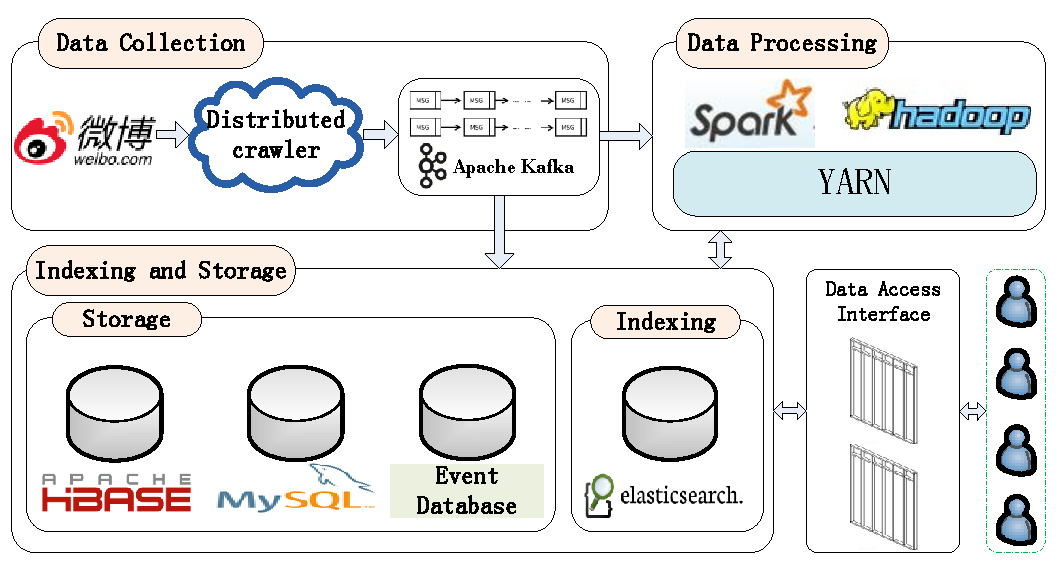
\includegraphics[scale=0.47]{system_architecture.pdf}
\centering
\caption{The Architecture of \ring System}
\label{fig:system_architecture}
\vspace{-3ex}
\end{figure}

As shown in Figure \ref{fig:system_architecture},
\ring system mainly consists of three modules, namely data collection, data indexing \& storage, and data processing.
%We implement a unified interface to process requests to these services.
For \emph{data collection}, we developed a distributed crawler to continuously fetch microblogs through Weibo API\footnote{http://open.weibo.com/wiki/Api}.
The collected data is forwarded to indexing and processing modules through Kafka\footnote{http://kafka.apache.org} to decouple their dependency.
For \emph{indexing and storage}, \ring utilizes HBase\footnote{http://hbase.apache.org/} and elasticsearch\footnote{https://github.com/elastic/elasticsearch} for data storage and full-text indexing, which is able to process large volumes of real-time microblog streams.
We further optimize elasticsearch over time range query for event tracking and query applications.
For \emph{data processing}, we implement our models and algorithms on Spark\footnote{http://spark.apache.org} and
 devise an optimization strategy for incremental statistics update to improve distributed processing efficiency.
